\documentclass[class=minimal,border=0pt]{standalone}
\usepackage{tikz}
\usepackage{amsmath, amsthm, amssymb}
\usetikzlibrary{arrows,shapes,trees}

\begin{document}
\pagestyle{empty}
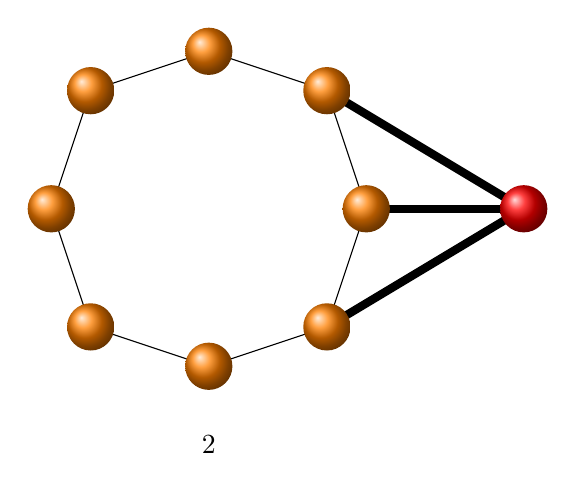
\begin{tikzpicture}
\path[draw] (0,0) -- (0.5,1.5) -- (2,2) -- (3.5,1.5) -- (4,0) -- (3.5,-1.5) -- (2,-2) -- (0.5,-1.5) -- cycle;
\path[draw,line width=3pt] (4,0) -- (6,0);
\path[draw,line width=3pt] (3.5,1.5) -- (6,0);
\path[draw,line width=3pt] (3.5,-1.5) -- (6,0);
\shade[shading=ball, ball color=orange] (0,0) circle (.3);
\shade[shading=ball, ball color=orange] (0.5,1.5) circle (.3);
\shade[shading=ball, ball color=orange] (2,2) circle (.3);
\shade[shading=ball, ball color=orange] (3.5,1.5) circle (.3);
\shade[shading=ball, ball color=orange] (4,0) circle (.3);
\shade[shading=ball, ball color=red] (6,0) circle (.3);
\shade[shading=ball, ball color=orange] (0.5,-1.5) circle (.3);
\shade[shading=ball, ball color=orange] (2,-2) circle (.3);
\shade[shading=ball, ball color=orange] (3.5,-1.5) circle (.3);
\draw  node[fill=white,circle,inner sep=0pt,minimum size=3pt] at (2,-3) {2} ;
\end{tikzpicture}

\end{document}
